\section{Background}
Poker software has been developed before by multiple companies, but these
are all mostly commercial, closed source software, with no discussion of the
algorithms and design decisions that went into them. This project will go
into depth on some of the issues that are faced when converting the game of
poker from the table to the computer.

%%%%%%%%%%%%%%%%%%%%%%%%%%%%%%%%%%%%%%
\subsection{Processes and Methodology}
%%%%%%%%%%%%%%%%%%%%%%%%%%%%%%%%%%%%%%

%%%%%%%%%%%%%%%%%%%%%%%%%%%%%%%%%%%%%
\subsection{Comparison of Algorithms}
%%%%%%%%%%%%%%%%%%%%%%%%%%%%%%%%%%%%%

Three different shuffling algorithms have been developed to examine in this
report. Here we will look about the differences between them, and the demand
upon memory and compute resources. We have three different card picking
algorithms, Knuth Shuffle, RandomSort Shuffle, and RandomIndex. RandomIndex
is unique in that instead of shuffling the deck, it picks a random card
from the deck on demand.

\vspace{0.3cm}

\begin{algorithm}[H]
    \SetKwInOut{Input}{input}\SetKwInOut{Output}{output}
    \Input{A deck of cards, $deck$}
    \Output{A shuffled deck of cards}
    \BlankLine{}
    \nlset{STEP 1} \For{$i \leftarrow 0$ \KwTo{} $len(deck)$}{
    \nlset{STEP 2}      $swap(deck, i, random(i, len(deck))$\;
                   }
\caption{The knuth shuffle algorithm}
\label{code:knuthshuffle}
\end{algorithm}

\vspace{0.3cm}

The first algorithm, the knuth shuffle, as seen in algorithm~\ref{code:knuthshuffle},
is very simple to understand, and produces a true shuffle, provided the
random number generator has at least 226 bits of internal state, to produce all
the possible permutations of a 52-card deck. ($52! \approx 2^{225.6}$) \parencite{arkin1999}

If the algorithm is implemented correctly, with the changes implemented by
\parencite{richard1964}, then the algorithm time complexity is reduced from
$O(n^2)$ to $O(n)$. In addition, this algorithm has a memory complexity of
$O(1)$.

\vspace{0.3cm}

\begin{algorithm}[H]
    \SetKwInOut{Input}{input}\SetKwInOut{Output}{output}
    \Input{A deck of cards, $deck$}
    \Output{A shuffled deck of cards}
    \BlankLine{}
    \nlset{STEP 1} $tmp \leftarrow []$\;
    \nlset{STEP 2} \For{$i \leftarrow 0$ \KwTo{} $len(deck)$}{
    \nlset{STEP 3}      $tmp[i] \leftarrow (i, random(0, RAND\_MAX)$\;
                   }
    \nlset{STEP 4} sortBy($tmp$, snd)\;
    \nlset{STEP 5} $deck \leftarrow map (fst) tmp$\;
\caption{The random sort shuffle algorithm}
\label{code:randomsort}
\end{algorithm}

\vspace{0.3cm}

The random sort shuffle, as seen in algorithm~\ref{code:randomsort} is not as
simple as the knuth shuffle, but still easy enough to understand. Each card
is assigned a random number, then the deck of cards is sorted based on the
random number. Due to Haskell being a lazy language, the complexity of this
algorithm is somewhat difficult to determine. The complexity of the sort
function is $O($n log k$)$, where k is the number of elements inspected. The
sort function is called on demand, so if a list is sorted, but never inspected,
no work is ever done. If only the first element is inspected, then the
complexity is $O(n)$. In the worst case, this algorithm is $O($n log n$)$.
This function has $O(n)$ memory usage, for the random numbers stored before
the list is sorted.

\vspace{0.3cm}

\begin{algorithm}[H]
    \SetKwInOut{Input}{input}\SetKwInOut{Output}{output}
    \Input{A deck of cards, $deck$}
    \Output{A random card}
    \BlankLine{}
    \nlset{STEP 1} return $deck[random(0, len(deck))]$\;
\caption{The random index card picking algorithm}
\label{code:randomsort}
\end{algorithm}

\vspace{0.3cm}

This random index card picking algorithm is the simplest of them all. It simply
picks a random card from the deck and returns it, on demand, instead of
shuffling the deck. This trades off an up front time cost for shuffling, for
a smaller, more frequent cost, when cards are needed. In most cases, this
total time should be smaller than shuffling the whole deck, as a full deck
of cards is not needed, except with a very large amount of players in the game
of poker. This algorithm has a complexity of $O(1)$, and a memory complexity
of $O(1)$.

%%%%%%%%%%%%%%%%%%%%%%%%%%%%%%%%%%
\subsection{Alternative Solutions}
%%%%%%%%%%%%%%%%%%%%%%%%%%%%%%%%%%

As previously mentioned, there are many different online poker software's
available. Here, we will look at some vendors offerings.

\begin{figure}[H]
    \frame{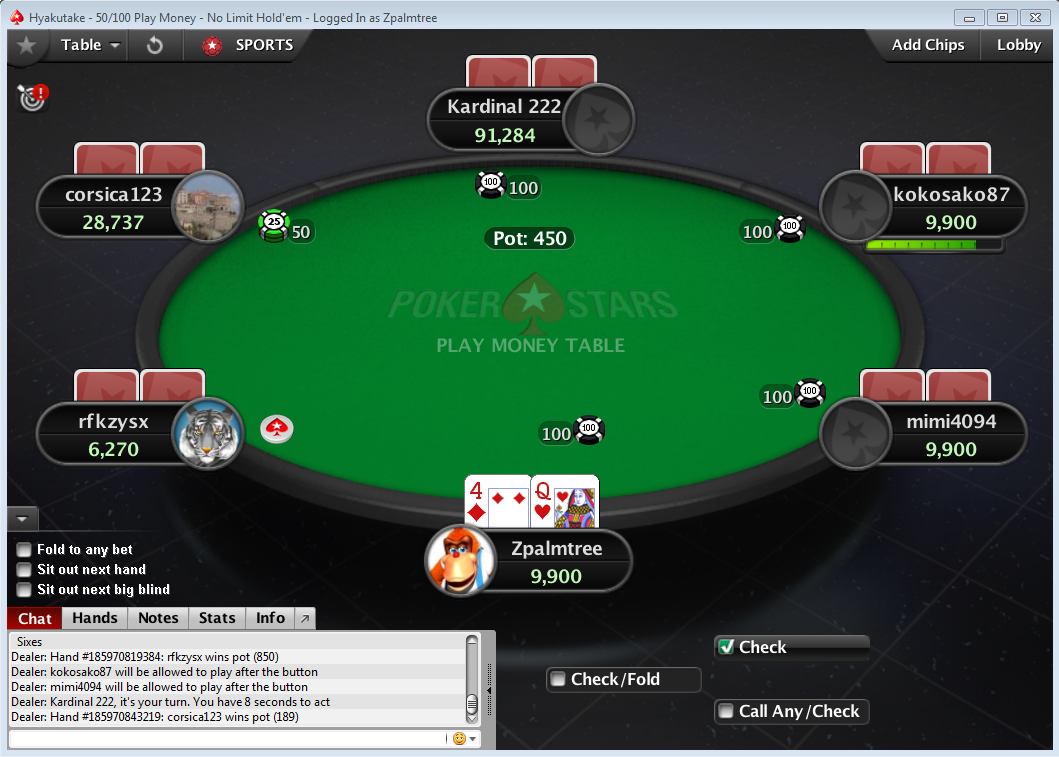
\includegraphics[width=\linewidth]{../images/pokerstars.png}}
    \caption{PokerStars poker software}%
    \label{fig:pokerstars}
\end{figure}

Figure~\ref{fig:pokerstars} shows the software produced by Poker Stars, one
of the leading poker software creators. Whilst the software itself is
featureful, and is available for Windows, macOS, Android, and iOS, the code
is closed source, and the shuffling algorithms or random number generator
implementation is not available for inspection. However, their RNG and its
implementation of the shuffling of cards has been verified by a third party,
Gaming Laboratories. \parencite{website:gaminglabs2015}

\begin{figure}[H]
    \frame{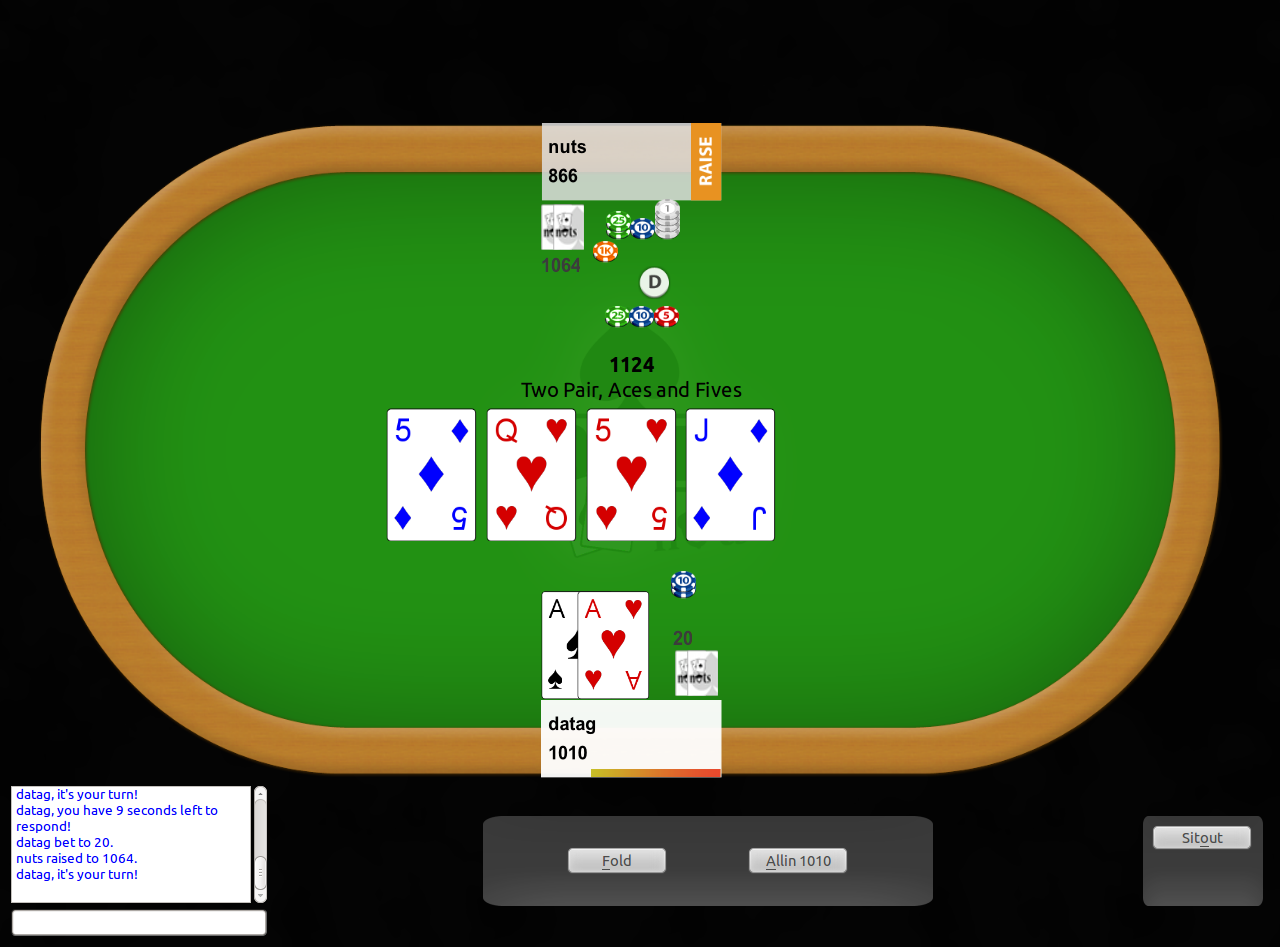
\includegraphics[width=\linewidth]{../images/holdingnuts.png}}
    \caption{HoldingNuts poker software}%
    \label{fig:holdingnuts}
\end{figure}

Figure~\ref{fig:holdingnuts} shows the software produced by Holding Nuts, an
open source poker client and server. Whilst this software is a lot less
advanced than the software offered by Poker Stars, due to it being open source,
we can inspect its shuffle algorithm, and random number generator. However,
upon inspecting the code, we find it simply uses the libpoker \parencite{code:dachary2004}
library, and only offers one shuffle, with one algorithm source.

Furthermore, whilst the code is open, the reasons behind implementation details
are not specified, so third parties may not understand the reason behind choices
of algorithms, and the subtleties involved to create a fair shuffle.

Whilst this software
is very helpful for people implementing open source clients, for people wishing
to develop closed source clients, the software is licensed under the GNU
GPL, and so they would be unable to use any code without also licensing their
code under the GPL\@.

%%%%%%%%%%%%%%%%%%%%%%%%%%%%%%%%%%%%%%%
\subsection{Comparison of Technologies}
%%%%%%%%%%%%%%%%%%%%%%%%%%%%%%%%%%%%%%%

\subsubsection{Programming Language}

The software developed for this report is relatively operating system and
programming language agnostic, and so multiple different ones were considered.

\begin{table}[H]
    \begin{adjustbox}{center}
    \begin{tabular}{l l l l l}
    \toprule
    Language             & Experience  & Type System            & Development Speed & Paradigm          \\
    \midrule
    Haskell              & Experienced & Strongly, Statically   & Medium            & Functional        \\ \addlinespace
    C\#                  & Experienced & Strongly, Statically   & Medium            & OOP               \\ \addlinespace
    Golang               & Low         & Strongly, Statically   & Slow              & Procedural        \\ \addlinespace
    C                    & Medium      & Weakly, Statically     & Slow              & Procedural        \\ \addlinespace
    Python               & Medium      & Strongly, Dynamically  & Fast              & OOP, Procedural   \\ \addlinespace
    C++                  & Medium      & Strongly, Statically   & Slow              & OOP, Procedural   \\ \addlinespace
    \bottomrule
    \end{tabular}
    \end{adjustbox}
    \caption{The differences of known programming languages}
\end{table}

It was decided to use a language with strong, static typing, due to this
class of typing preventing a large class of bugs at runtime, instead being
caught at compile time. This left Haskell, C\#, Golang, and C++. To narrow it
down, the languages the developer was less experienced in were abandoned,
and out of Haskell and C\#, Haskell was chosen, due to the functional paradigm
leading to ease of testing smaller isolated modules, high levels of code
reuse, and less bugs, due to immutable state.

\subsubsection{GUI Toolkit}

Once a programming language had been decided on, a library to develop the
graphical user interface was needed. Some of these libraries only run on
certain operating systems, and have different levels of difficulty and
boilerplate code required to use them.

\begin{table}[H]
    \begin{adjustbox}{center}
    \begin{tabular}{l l l l}
    \toprule
    GUI Toolkit & Language Interface    & Development Speed & Supported OS's        \\
    \midrule
    GTK         & Haskell               & Medium            & Linux, OSX            \\ \addlinespace
    QtQuick     & Javascript + Haskell  & Fast              & Linux, OSX, Windows   \\ \addlinespace
    wxWidgets   & Haskell               & Medium            & Linux, OSX, Windows   \\ \addlinespace
    SDL2        & Haskell               & Slow              & Linux, OSX, Windows   \\ \addlinespace
    \bottomrule
    \end{tabular}
    \end{adjustbox}
    \caption{The differences of possible GUI toolkits}
\end{table}

All of the toolkits looked at have a Haskell library interface, as is needed
to work with the rest of the code. QtQuick however is unique in that the GUI
interface is written in JavaScript, then the interactions with it can be
programmed from both JavaScript and/or Haskell. Due to Haskell being a language
that has immutable by default variables, it is often cumbersome to utilise
graphical libraries, however, with QtQuick, the GUI can be quickly prototyped
in JavaScript, and then the GUI data (cards, player names, etc), can be filled
from the Haskell side. Due to the amount of GUI code being quite minimal, the
weakly typed JavaScript is not much of an issue to debug. For these reasons,
QtQuick was chosen for the GUI framework.

%%%%%%%%%%%%%%%%%%%%%%%%%%%%%%%%%%%%%%%%%%%%%%%
\subsection{Problem Context}
%%%%%%%%%%%%%%%%%%%%%%%%%%%%%%%%%%%%%%%%%%%%%%%

\subsubsection{Randomness}
In this report we will talk a lot about different random sources. By this we
mean a library of function that provides random numbers, using a certain
algorithm. Each of these algorithms have a few properties that set them apart
from different ones, most notably:

\begin{itemize}
\item Bit Size
\item Cycle Length
\end{itemize}

When we generate random numbers, we use a pseudo random number generator
(Henceforth prng). These
use an algorithm to determine a number from the previous one, and they all
eventually loop back to the start of the cycle. If we provide a seed to one
of these generators, it provides us a set start point into the generator, after
which the sequence of random numbers is always the same. This can be helpful
to reproduce exact program results, for example for debugging. If the seed
size is for example, 8 bits, then there are only 256 possible beginnings to
the sequence. Therefore, when we create and seed our generator, whilst it may
appear that we are getting lots of different random numbers, we are only
in fact getting 256 different sequences of numbers. One way to avoid this is
by reseeding the generator between each call of the prng, however this is
generally very slow, and so not viable in performant applications. For
simplicity, if we say that the prng is seeded at the beginning of each shuffle,
we can therefore generate only the amount of shuffles as the size of our seed,
whilst there are
$52! = 80658175170943878571660636856403766975289505440883277824000000000000$
possible shuffles. Some shuffles however, use much larger internal bit sizes than
the bit size of the outputs, for example, Multiply With Carry 256 \parencite{marsaglia2003}
uses an internal bit size of 256 bits as the name suggests.

Secondly we can talk about the cycle length. This is the period that the prng
lasts for, before the numbers start repeating. For example, if we had a prng
with a cycle length of 10, we would be able to get 10 random numbers, before
the generator would loop back to the first of the ten random numbers again.
Most modern generators have very large cycle lengths, but this should be taken
care of, as if the usage of the random number generator is predictable, after
a system has been online for a long time, it is possible to predict new values
based on previous values.

\subsubsection{The Game of Poker}
Each player is dealt two cards, and the player to the left of the dealer must
pay a small bet, called the small blind, with the player to his left paying 
double this bet, the big blind. Play then proceeds clockwise from the next
player. Each player has the option to fold, check, call, raise, or go all in,
depending upon the circumstances. Folding forfeits any stake in the round, and
removes you from play. Checking means you wish not to bet, and is only
available if there is no current bet which needs matching. Calling means to
match the current bet, and raising means to raise the current bet to a higher
value. Going all in means to bet all your chips, and sometimes is mandatory to
remain in the pot, if you have less chips than the current bet. This can cause
multiple side pots to occur. Each player has an amount of chips at the 
beginning of the game which they bet with, these may be backed by real money as
is the case in casinos and most online poker software. Once all players have
matched the current bet or folded, three table cards are revealed, called
the flop. These are common to all players hands, and may be used along with
the players two hidden cards to form the best 5 card hand. A further two table
cards will be revealed as play continues, unless all players but one fold,
leaving the winner to keep any bet chips. Again, players may bet if they wish.
Providing there are still players in play, the fourth card will be revealed, 
called the turn. The same process occurs again, then the fifth card will be
revealed, the river. Once this betting round has ended, any players still
in play reveal their cards, and the winner is the player who has the best
five card hand. These can vary from simple pairs, to higher valued hands such
as a straight, which is five cards in a row, such a 5, 6, 7, 8, 9. The winner
receives all the chips in the middle of the table gained from other players
bets, and a new round begins, with the dealer moving to the next player on the
left.
